\textcolor{blue}{\textit{Maxime Bouyssou}}



\subsection{Hardware architecture}
The hardware part of each robot is pretty simple. Each robot is equipped with a serial GPS wired to a serial radio module (see figure below). So each robots will emits its GPS coordinates to the central computer who will then uses this coordinates to compute the next order he will send to them.

\begin{center}
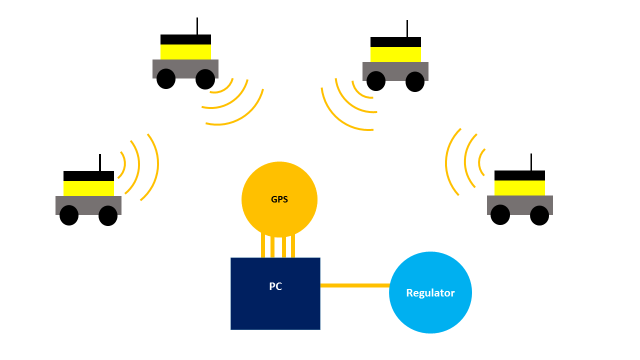
\includegraphics[scale=0.2]{GPS_emit.png} 
\captionof{figure}{Robot emitting their GPS coordinates}
\label{fig1}
\end{center}

The radio modules are wired to the power electronic parts of the robot. The robot is controlled via a standard RC radio link. The idea is that the central computer can directly send his orders via the radio transmission to the robots. (see figure below)

\begin{center}
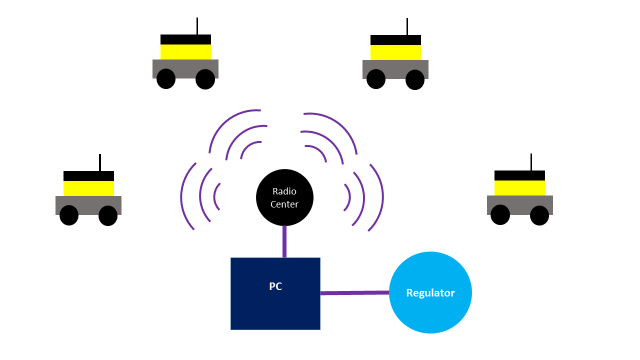
\includegraphics[scale=0.2]{Radio_control.png} 
\captionof{figure}{Robot emitting their GPS coordinates}
\label{fig1}
\end{center}

Here is a more details view of all the composants inside the robots.

\begin{center}
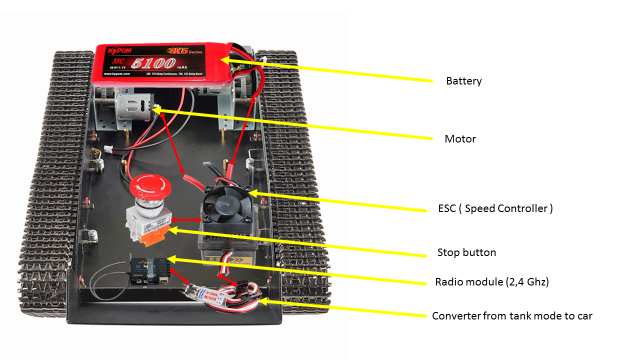
\includegraphics[scale=0.2]{robot.png} 
\captionof{figure}{Construction of the robot	}
\label{fig1}
\end{center}

Here is a more details view of all the composants on the ground station

\begin{center}
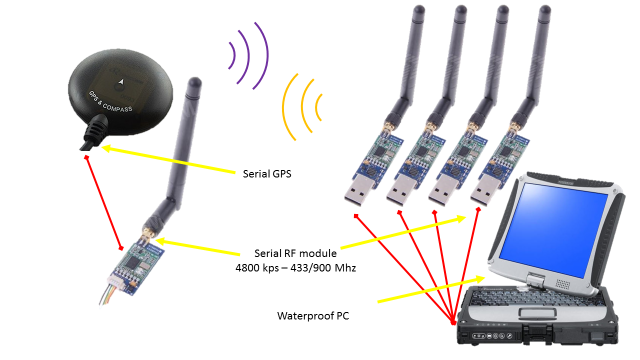
\includegraphics[scale=0.2]{GPS.png} 
\captionof{figure}{GPS}
\label{fig1}
\end{center}

\begin{center}
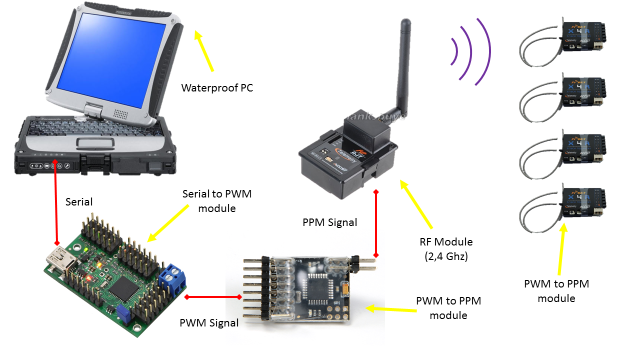
\includegraphics[scale=0.2]{stationControl.png} 
\captionof{figure}{Station Control}
\label{fig1}
\end{center}